\documentclass{cmc}

\hypersetup{
    colorlinks=true,
    linkcolor=blue,
    filecolor=magenta,
    urlcolor=red,
}
\urlstyle{same}

\begin{document}
\maketitle
\pagestyle{fancy}
\tableofcontents
\lhead{\textit{\textbf{Computational Motor Control, Spring 2019} \\
    Python exercise, Lab 0, NOT GRADED}} \rhead{Student \\ Names}

\newpage
\section*{Student names: \ldots (please update)}

\textit{Instructions: This document contains the instructions to
  install and get familiarized with Python programming.  \textbf{This
    lab is not graded}. This file does not need to be submitted and is
  provided for your own benefit.}


\section{Course Organization}

This year all the exercises for the course will be distributed through
\href{https://gitlab.epfl.ch/}{EPFL's GitLab}.  GitLab is an online
open source Git repository for maintaining and distributing code
between groups of people. The access to the exercises repository is
public and you can directly use your epfl credentials to login.  We
recommend you to use the features Git offers to collaborate with your
partners and maintain a history of your own work as well.  If you
download the repository without cloning, then you will have to do it
every week and you will end up downloading all the previous files
every time you do it. This report does not contain a tutorial on how
to use Git but you can find the references in section
\ref{sec:git_ref}. However, we will have short demo on how to use it
during the exercise hour.

The link to the \href{https://gitlab.epfl.ch/BioRobCMC/2019}{git
  repository}

This course expects you to complete the exercises using the standard
Python programming language. There are many options to use Python. For
those students who are starting of new with Python, we strongly
suggest to follow the following installation steps.
\textbf{\corr{NOTE : }}\textit{All the Python codes provided in this
  lab should be studied carefully as these basic notions will be
  needed in the future exercises and projects of this course.}

\textbf{\corr{NOTE : }}\textit{The course supports the use of Python 3
  unless otherwise mentioned.}

\section{Windows}
\label{sec:windows}

\subsection{Python}
\label{sec:python-win}
\subsubsection{Checking if python exists}
\label{sec-win:checking-if-python}
Before installing please check if you already have python installed on
your computer.  To do so open Git Bash (Application you must have
already installed while following the Git Instructions document)

Once Git Bash is open execute the following commands,

\begin{lstlisting}[language=bash]
$ python -V
\end{lstlisting}
\begin{lstlisting}[language=bash]
$ python3 -V
\end{lstlisting}

If either of them returns \verb|Python 3| then you can skip the Python
installation section and continue with the rest.

\subsubsection{Installation}
\label{sec-win:installation-python}

To download and install Python use the link :
\href{https://www.python.org/downloads/windows/}{Python-Windows}

During installation, when you see the pop up window figure
 \ref{fig:win-py-step1} make sure you check on the box \textit{Add
  Python 3.7 to PATH} and you click on the customize installation
option.

Next, you will see figure \ref{fig:win-py-step2} where you need to make sure
all the check boxes are ticked. Finally in the advanced options step
like figure \ref{fig:win-py-step3} you need to tick the choices like shown in
the figure unless you are sure you know the implications of your
choices.

\begin{figure}[H]
  \centering
  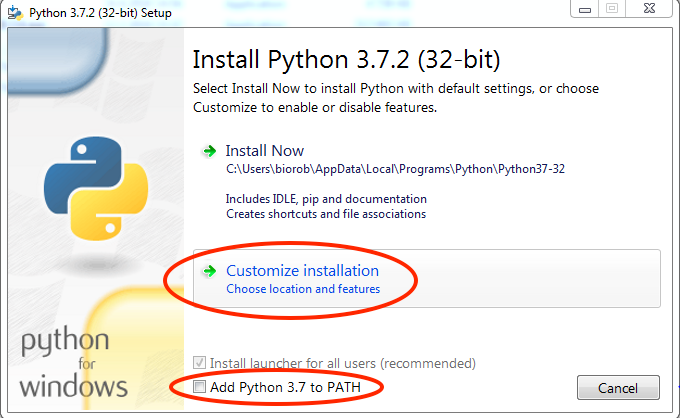
\includegraphics[width=\textwidth]{figures/python_install_1}
  \caption{Python installation customization - Step 1}
  \label{fig:win-py-step1}
\end{figure}

\begin{figure}[H]
  \centering
  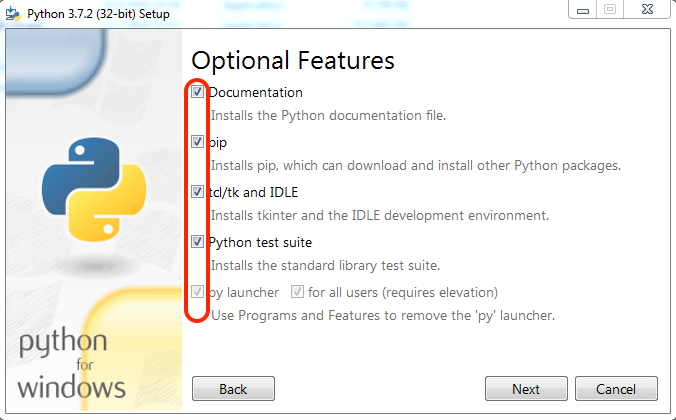
\includegraphics[width=\textwidth]{figures/python_install_2}
  \caption{Python installation customization - Step 2}
  \label{fig:win-py-step2}
\end{figure}

\begin{figure}[H]
  \centering
  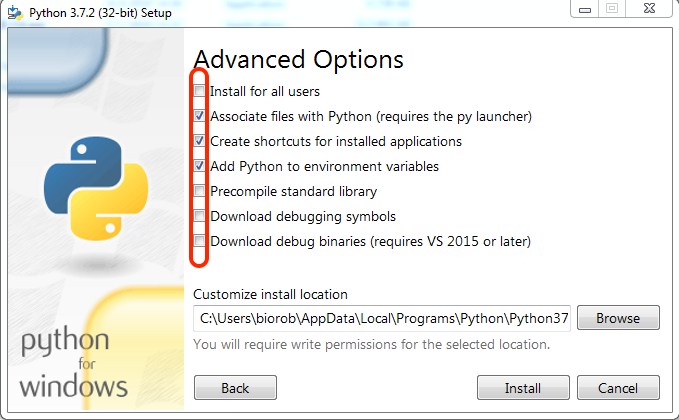
\includegraphics[width=\textwidth]{figures/python_install_3}
  \caption{Python installation customization - Step 3}
  \label{fig:win-py-step3}
\end{figure}

\textbf{\corr{NOTE : }}\textit{Install 3.7.2}

After installation to verify if everything is working open Git Bash
again and run the above commands to check the python versions.

\subsection{Pip}
\label{sec-win:pip}

Python has a huge repository of packages that are widely used for
different functions. In order to obtain these packages there are
several package managers. The one we will be using during this course
will be the official package installer for Python called $pip$.

\subsubsection{Checking if pip exists}
\label{sec-win:checking-if-pip}

If you installed Python based on the instructions above then pip
should be installed by default. Or it may have been already installed
on your computer if Python had been pre-installed. To check if pip
exists, open Git Bash and execute the following command:

\textbf{\corr{NOTE : }}\textit{$pip$ or $pip3$ depends on your
  system. Typically they differentiate ones installed with python2 and
  python3 respectively.}

\begin{lstlisting}[language=bash]
$ pip --version
\end{lstlisting}

\begin{lstlisting}[language=bash]
$ pip3 --version
\end{lstlisting}

If
$pip$ is already installed then at least one of the above commands
should print the version of the pip along with the python and its
version associated with it. \textbf{Make sure that the python version
  is $3$}

\subsubsection{Installation}
\label{sec-win:installation-pip}
If you have verified that pip is not installed on your computer then
in order to install pip you are expected to have either cloned or
downloaded the exercise repository by now.
\begin{itemize}
\item Open Git Bash
\item Navigate to the location where you have downloaded the exercise
  repository. You can use the command $cd$ to change directories and
  $pwd$ to check you current directory.
\item Inside the exercise repository navigate to
  \textbf{\textit{extras}} folder and execute the following command:
\end{itemize}

\begin{lstlisting}[language=bash]
$ python get-pip.py
\end{lstlisting}

\textbf{\corr{NOTE : }}\textit{Make sure command \textbf{python}
  refers to python-3. To check use the commands mentioned in Python
  Installation section to get the corresponding python version.
  Accordingly use either python or python3 commands}

Check if you have installed everything correctly by referring to
\ref{sec-win:checking-if-pip}.

\subsection{Spyder}
\label{sec-win:spyder}

Python programs can be written and run in several ways, it can be
simply done on a terminal by running \textit{python} or
\textit{ipython}. While this method is limited for simple programs,
larger programs will be written using a text-editor or an Integrated
Development Environment (IDE). Though it is not necessary to have an
IDE for programming in Python, having one will bring many features
that are useful while starting new

\subsubsection{Installation}
\label{sec-win:installation-spyder}

\begin{itemize}
\item Open Git Bash
\item Execute the following command:
\begin{lstlisting}[language=bash]
$ pip install pyqt5==5.9.2
\end{lstlisting}
  or
\begin{lstlisting}[language=bash]
$ pip3 install pyqt5==5.9.2
\end{lstlisting}
  Use of $pip$ or $pip3$ depends on the one associated with python3.
  If you are not sure refer back to section
  \ref{sec-win:checking-if-pip}
\item Next, install spyder with the command:
\begin{lstlisting}[language=bash]
$ pip install spyder
\end{lstlisting}
  or
\begin{lstlisting}[language=bash]
$ pip3 install spyder
\end{lstlisting}
\end{itemize}

\subsubsection{Checking spyder}
\label{sec-win:checking-if-spyder}

To check if spyder is installed, execute the following command from
Git Bash

\begin{lstlisting}[language=bash]
$ spyder3
\end{lstlisting}

If everything is working then Spyder IDE should open and you are ready
to begin with the exercises.

\newpage
\section{Mac-OSX}
\label{sec:mac}

\subsection{Python}
\label{sec-mac:python}
\subsubsection{Checking if python exists}
\label{sec-mac:checking-if-python}
Before installing please check if you already have python installed on
your computer. To do so open terminal application.  Once terminal is
open execute the following commands,
\begin{lstlisting}[language=bash]
$ python -V
\end{lstlisting}
\begin{lstlisting}[language=bash]
$ python3 -V
\end{lstlisting}

If either of them return \verb|Python 3| then you can skip the Python
installation section and continue with the rest.

\subsubsection{Installation}
\label{sec-mac:installation-python}

To download and install Python use the link :
\href{https://www.python.org/downloads/mac-osx/}{MacOS}

During installation step make sure you choose customize option like in
figure \ref{fig:mac-py-step1} and then confirm that all the check
boxes are selected like in figure \ref{fig:mac-py-step2}

\begin{figure}[H]
  \centering
  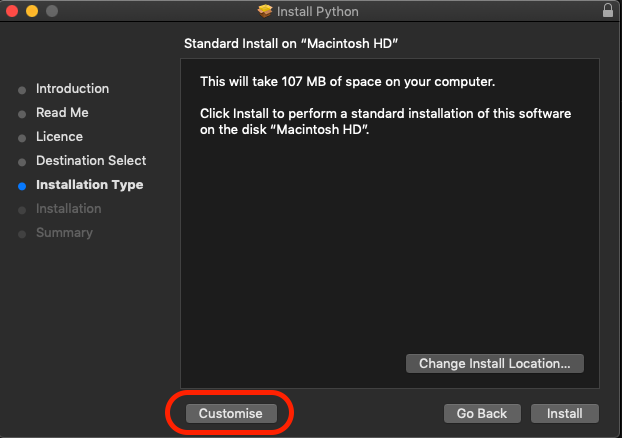
\includegraphics[width=\textwidth]{figures/python_install_4}
  \caption{Python installation customization - Step 1}
  \label{fig:mac-py-step1}
\end{figure}

\begin{figure}[H]
  \centering
  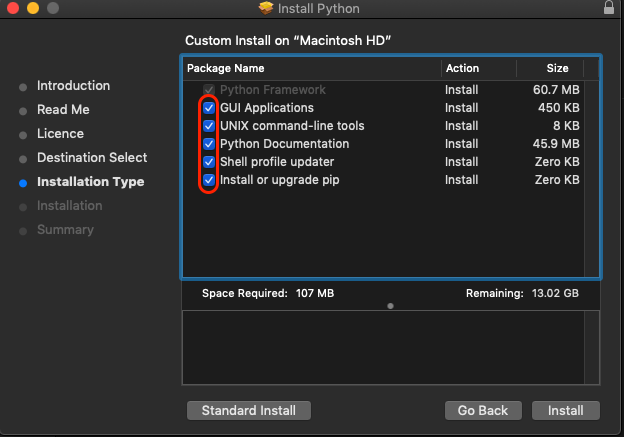
\includegraphics[width=\textwidth]{figures/python_install_5}
  \caption{Python installation customization - Step 2}
  \label{fig:mac-py-step2}
\end{figure}


\textbf{\corr{NOTE : }}\textit{Install 3.7.2}

After installation to verify if everything is working open terminal
again and run the commands in section
\ref{sec-mac:checking-if-python}.

\subsection{Pip}
\label{sec-mac:pip}

Python has a huge repository of packages that are widely used for
different functions. In order to obtain these packages there are
several package managers. The one we will be using during this course
will be the official package installer for Python called $pip$.

\subsubsection{Checking if pip exists}
\label{sec-mac:checking-if-pip}

If you installed Python based on the instructions above then pip
should be installed by default. Or it may have been already installed
on your computer if Python had been pre-installed. To check if pip
exists, open terminal and execute the following command:

\textbf{\corr{NOTE : }}\textit{$pip$ or $pip3$ depends on your
  system. Typically they differentiate ones installed with python2 and
  python3 respectively.}

\begin{lstlisting}[language=bash]
$ pip --version
\end{lstlisting}

\begin{lstlisting}[language=bash]
$ pip3 --version
\end{lstlisting}

If
$pip$ is already installed then at least one of the above commands
should print the version of the pip along with the python and its
version associated with it. \textbf{Make sure that the python version
  is $3$}

\subsubsection{Installation}
\label{sec-mac:installation-pip}
If you have verified that pip is not installed on your computer then
in order to install pip you are expected to have either cloned or
downloaded the exercise repository by now.
\begin{itemize}
\item Open terminal application
\item Navigate to the location where you have downloaded the exercise
  repository. You can use the command $cd$ to change directories and
  $pwd$ to check you current directory.
\item Inside the exercise repository navigate to
  \textbf{\textit{extras}} folder and execute the following command:
\end{itemize}

\begin{lstlisting}[language=bash]
$ python get-pip.py
\end{lstlisting}

\textbf{\corr{NOTE : }}\textit{Make sure command \textbf{python}
  refers to python-3. To check use the commands mentioned in Python
  Installation section to get the corresponding python version.
  According use either python or python3 commands}

Check if you have installed everything correctly by referring to
\ref{sec-mac:checking-if-pip}.

\subsection{Spyder}
\label{sec-mac:spyder}

Python programs can be written and run in several ways, it can be
simply done on a terminal by running \textit{python} or
\textit{ipython}. While this method is limited for simple programs,
larger programs will be written using a text-editor or an Integrated
Development Environment (IDE). Though it is not necessary to have an
IDE for programming in Python, having one will bring many features
that are useful while starting new

\subsubsection{Installation}
\label{sec-win:installation-spyder}

\begin{itemize}
\item Open terminal
\item Execute the following command:
\begin{lstlisting}[language=bash]
$ pip install pyqt5==5.9.2
\end{lstlisting}
  or
\begin{lstlisting}[language=bash]
$ pip3 install pyqt5==5.9.2
\end{lstlisting}
  Use of $pip$ or $pip3$ depends on the one associated with python3.
  If you are not sure refer back to section
  \ref{sec-mac:checking-if-pip}
\item Next, install spyder with the command:
\begin{lstlisting}[language=bash]
$ pip install spyder
\end{lstlisting}
  or
\begin{lstlisting}[language=bash]
$ pip3 install spyder
\end{lstlisting}
\end{itemize}

\subsubsection{Checking spyder}
\label{sec-mac:checking-if-spyder}

To check if spyder is installed, execute the following command from a
terminal.

\begin{lstlisting}[language=bash]
$ spyder3
\end{lstlisting}

If everything is working then Spyder IDE should open and you are ready
to begin with the exercises.

\newpage
\section{Linux}
\label{sec:lin}

\textbf{\corr{NOTE : }}\textit{These instruction are for Ubuntu or
  other Debian-based distributions. The setup for other Linux
  distributions should be adapted accordingly.}

\subsection{Python}
\label{sec-lin:python}
\subsubsection{Checking if python exists}
\label{sec-lin:checking-if-python}
Before installing please check if you already have python installed on
your computer. To do so open terminal application.  Once terminal is
open execute the following commands,
\begin{lstlisting}[language=bash]
$ python -V
\end{lstlisting}
\begin{lstlisting}[language=bash]
$ python3 -V
\end{lstlisting}

If either of them return \verb|Python 3| then you can skip the Python
installation section and continue with the rest.

\subsubsection{Installation}
\label{sec-lin:installation-python}

To download and install Python use the link :
\begin{itemize}
\item Open terminal application
\item Execute the following command:
\begin{lstlisting}[language=bash]
$ sudo apt-get install python3
\end{lstlisting}
  The above command will ask you to enter your system password before
  beginning the installation process.
\end{itemize}

After installation to verify if everything is working open terminal
again and run the commands in section
\ref{sec-lin:checking-if-python}.

\subsection{Pip}
\label{sec-lin:pip}

Python has a huge repository of packages that are widely used for
different functions. In order to obtain these packages there are
several package managers. The one we will be using during this course
will be the official package installer for Python called $pip$.

\subsubsection{Checking if pip exists}
\label{sec-lin:checking-if-pip}

If you installed Python based on the instructions above then pip
should be installed by default. Or it may have been already installed
on your computer if Python had been pre-installed. To check if pip
exists, open terminal and execute the following command:

\textbf{\corr{NOTE : }}\textit{$pip$ or $pip3$ depends on your
  system. Typically they differentiate ones installed with python2 and
  python3 respectively.}

\begin{lstlisting}[language=bash]
$ pip --version
\end{lstlisting}

\begin{lstlisting}[language=bash]
$ pip3 --version
\end{lstlisting}

If
$pip$ is already installed then at least one of the above commands
should print the version of the pip along with the python and its
version associated with it. \textbf{Make sure that the python version
  is $3$}

\subsubsection{Installation}
\label{sec-lin:installation-pip}
If you have verified that pip is not installed on your computer then
in order to install pip you are expected to have either cloned or
downloaded the exercise repository by now.
\begin{itemize}
\item Open terminal application
\item Execute the following command:
\begin{lstlisting}[language=bash]
$ sudo apt-get install python3-pip
\end{lstlisting}
\end{itemize}

Check if you have installed everything correctly by referring to
\ref{sec-lin:checking-if-pip}.

\subsection{Spyder}
\label{sec-mac:spyder}

Python programs can be written and run in several ways, it can be
simply done on a terminal by running \textit{python} or
\textit{ipython}. While this method is limited for simple programs,
larger programs will be written using a text-editor or an Integrated
Development Environment (IDE). Though it is not necessary to have an
IDE for programming in Python, having one will bring many features
that are useful while starting new

\subsubsection{Installation}
\label{sec-lin:installation-spyder}

\begin{itemize}
\item Open terminal
\item Execute the following command:
\begin{lstlisting}[language=bash]
$ pip install pyqt5==5.9.2
\end{lstlisting}
  or
\begin{lstlisting}[language=bash]
$ pip3 install pyqt5==5.9.2
\end{lstlisting}
  Use of $pip$ or $pip3$ depends on the one associated with python3.
  If you are not sure refer back to section
  \ref{sec-lin:checking-if-pip}
\item Next, install spyder with the command:
\begin{lstlisting}[language=bash]
$ pip install spyder
\end{lstlisting}
  or
\begin{lstlisting}[language=bash]
$ pip3 install spyder
\end{lstlisting}
\end{itemize}

\subsubsection{Checking spyder}
\label{seclin:checking-if-spyder}

To check if spyder is installed, execute the following command from a
terminal

\begin{lstlisting}[language=bash]
$ spyder3
\end{lstlisting}

If everything is working then Spyder IDE should open and you are ready
to begin with the exercises.

\newpage
\section{Spyder}
\label{sec:spyder}
Spyder can be run by executing the command \textit{spyder}.

Figure \ref{fig:spyder} shows the main windows when you first open
Spyder. As you may have noticed, the layout is similar to
Matlab. Spyder has very good documentation to get you started.  It is
recommended to go through the steps to get familiarized with the IDE.

\begin{figure}[h]
  \centering 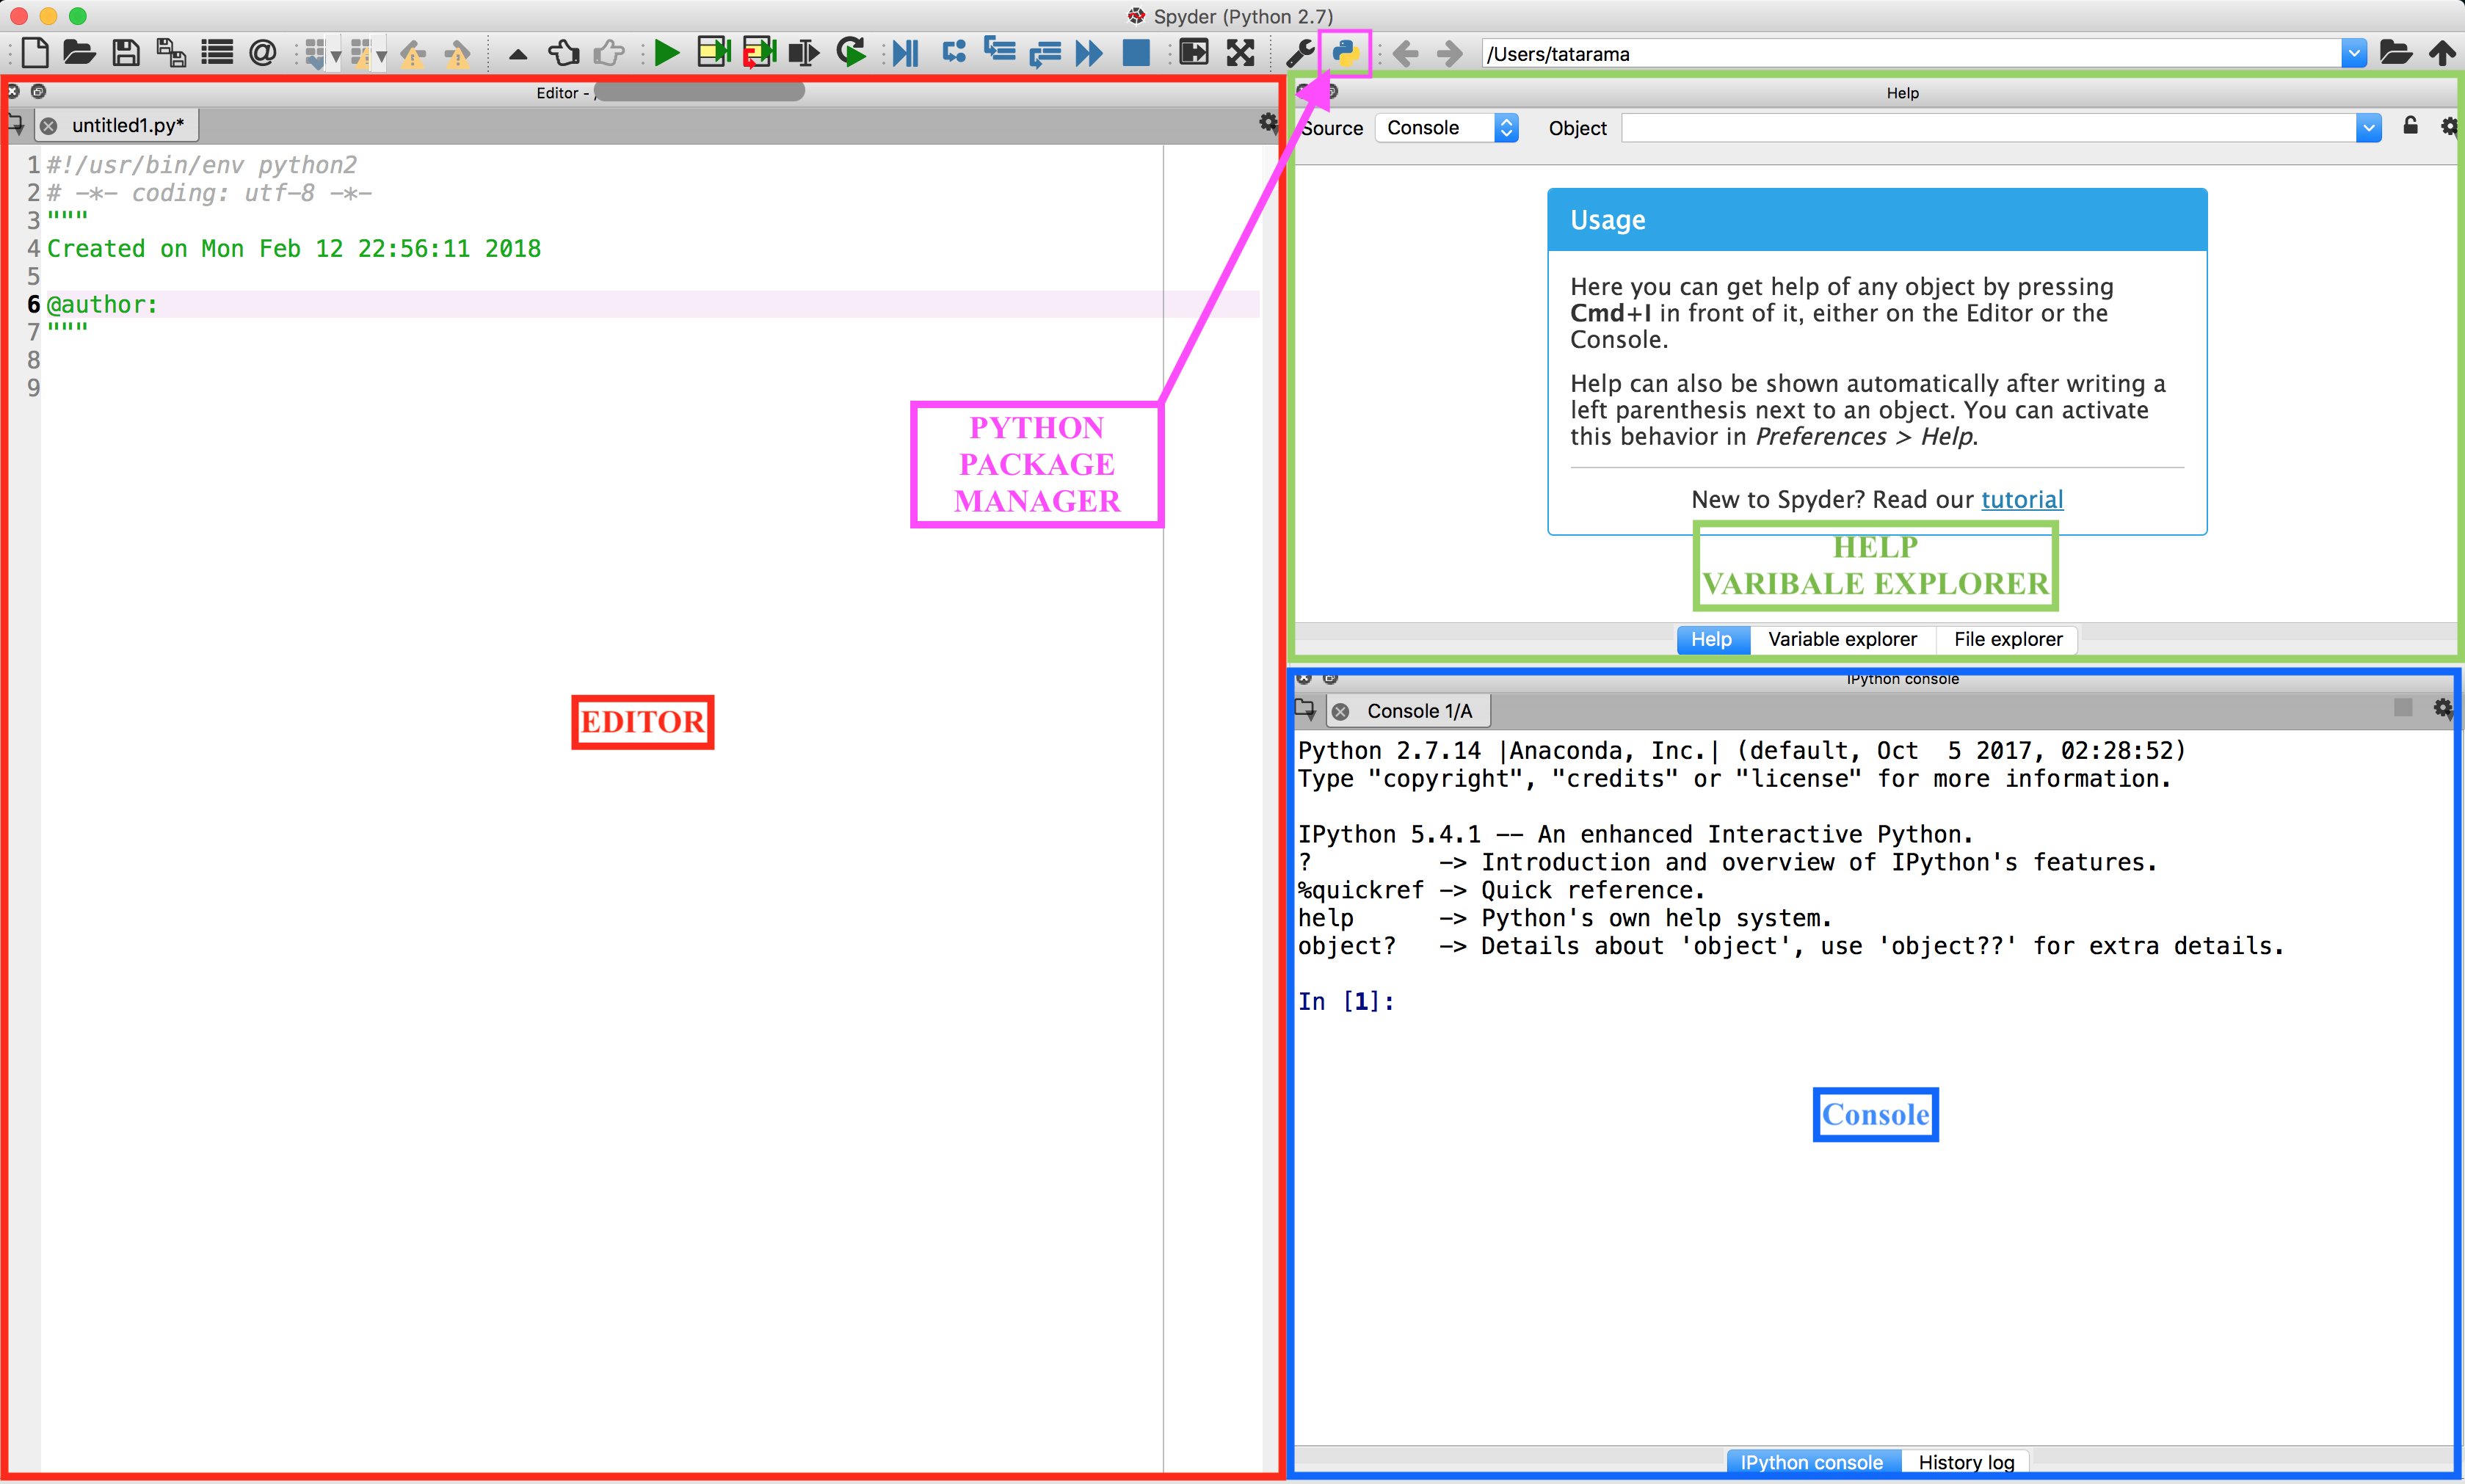
\includegraphics[width = \textwidth]{figures/Spyder.png}
  \caption{Spyder IDE overview}
  \label{fig:spyder}
\end{figure}

The three essential parts of the screen are outlined.

\begin{itemize}
\item \textbf{The console} (bottom right, marked in blue). You can
  work interactively here. Code run, either interactively or from the
  editor, will output any results here.  Error messages will be
  reported here. There are two types of console: a Python console, and
  an IPython console. Both will run Python code, but we recommend the
  IPython console as it offers better visuals for debugging and has
  additional features.
\item \textbf{The editor} (left, marked in red). You can write code to
  be saved to file or run here. This will suggest problems with syntax
  and has features to help debug and give additional information.
\item \textbf{The inspector} (top right, marked in green). The Object
  inspector can display detailed help on specific objects (or
  functions, or...), and the Variable inspector can display detailed
  information on the variables that are currently defined. Extremely
  useful when debugging.
\item \textbf{Python Package Manager} (top toolbar, marked in pink)
  Use this menu to add new paths to the default python package
  paths. (NOTE : The symbol may look slightly different on your
  machine from the one shown in this report)
\end{itemize}

For an in depth tutorial of Spyder follow the
\href{http://www.southampton.ac.uk/~fangohr/blog/spyder-the-python-ide.html#first-steps-with-spyder}{link}.

\subsection{Getting Help}
\label{sec:getting-help}
In any python console you can get information about a particular
python object using the \textit{help} method. For example to get help
on the type float,
\begin{lstlisting}[language=python]
help(float)
\end{lstlisting}
In spyder you can use this method in the console window.  The Spyder
environment also provides a panel in the top right corner (by default)
which is the Object inspector. If you type float into the empty line
in the Object inspector window, it will also provide the help string.

\subsection{Debugging}
\label{sec:debugging}
Refer to the link
\href{http://www.southampton.ac.uk/~fangohr/blog/spyder-the-python-ide.html#line-by-line-step-execution-of-code}{debug}

\newpage
\section{Programming with Python}

\subsection{Package installation}
\label{sec:package-installation}

The final step before starting of with the exercise is to install a
few necessary packages. We will be using pip to this.

\begin{itemize}
\item Open terminal (Git Bash on Windows)
\item Navigate in the terminal to the exercise repository on your
  computer
\item Execute the following command once you are in the root of the
  repository:
\begin{lstlisting}[language=bash]
$ pip install -r requirements.txt
\end{lstlisting}
  or
\begin{lstlisting}[language=bash]
$ pip3 install -r requirements.txt
\end{lstlisting}
  \textit{Use $pip$ or $pip3$ depending on the one that refers to
    python3.}
\end{itemize}

The \textit{requirements.txt} installs the following packages:
\begin{itemize}
\item numpy : Scientific computing package for python
\item matplotlib : Matlab like plotting tool for python
\item cmc\_pylog : Module for logging written for cmc
\end{itemize}


After successfully completing the installation steps in the previous
sections, you can now get started with programming using Python.
Python is not just a computational tool but a very powerful
programming language. This means having to learn a few more extra
concepts to get your job done.  There are a ton of references
available online for those who are interested in learning Python in
depth. We will try to provide the necessary references to help with
the concepts that are useful during the course as and when needed.

\subsection{Basic Python Concepts}

In this section we will quickly go over the list of topics given
below.  You can open and run the individual files marked with the same
topic name using Spyder.  We suggest you to go through each section
individually and spend time exploring each of the concepts by making
changes to the code and observing the outputs.

\begin{enumerate}
  \setcounter{enumi}{-1}
\item HelloWorld
\item Imports
\item Data Types
\item Math
\item Conditional Statements
\item Data Containers : Lists, Tuples and Dictionaries
\item Functions
\item Loops
\item Numpy
\item Matplotlib
\item Classes
\end{enumerate}

While you are executing each of the small exercises, try to learn how
to use different features of Spyder. Especially the help and debugging
feature.  When you are unsure of any command, use the help service
either the one built into Python or Spyder.  After familiarizing
yourself with the above concepts try to solve the following python
exercises.

\newpage
\subsection{Exercise 1}
\textbf{Check if the following matrix M is a magic square or not?}

\textit{\textbf{Hint : } A magic square is a square matrix which
  contains distinct integers and whose sum along any of its individual
  rows or columns or diagonal is a constant.  The constant is called
  as a magic constant or magic sum or magic square}

\begin{equation*}
  \label{eq:1}
  M =
  \begin{bmatrix}
    16 & 3  & 2  & 13 \\
    5  & 10 & 11 & 8  \\
    9  & 6  & 7  & 12 \\
    4 & 15 & 14 & 1
  \end{bmatrix}
\end{equation*}

\textit{\textbf{Further Step : } Try if you can generalize your script
  to have a function to check any arbitrary matrix if it is a magic
  square or not.  Import the function as a module in another script
  and use it to check the matrix M}

\subsection{Exercise 2 - Plotting a function}

\textit{Plot the following function $f(x)$ over an interval [0, 2]
  with proper labels and title}

\begin{equation*}
  \label{eq:3}
  f(x) = sin(x - 2)e^{-x^2}
\end{equation*}

\newpage
\section{References and additional useful links}
\label{sec:references}

\subsection{Python}
\label{sec:python_ref}
\begin{itemize}
\item
  \href{http://mathesaurus.sourceforge.net/matlab-numpy.html}{NumPy
    for MATLAB users}
\item \href{https://python.swaroopch.com}{A byte of python}
\item \href{http://nbviewer.jupyter.org/gist/rpmuller/5920182}{A Crash
    Course in Python for Scientists}
\item The official \href{https://docs.python.org/2/}{Python
    documentation} should be your first stop when looking for
  information
\item \href{http://numpy.scipy.org/}{numpy}
\item \href{http://www.scipy.org/}{scipy}
\item \href{http://matplotlib.sourceforge.net/}{matplotlib}
\end{itemize}

\subsection{Git}
\label{sec:git_ref}
\begin{itemize}
\item \href{https://try.github.io/levels/1/challenges/1}{Try Git!}
\item
  \href{https://marklodato.github.io/visual-git-guide/index-en.html}{A
    Visual Git Reference}
\end{itemize}

\subsection{Spyder}
\label{sec:spyder_ref}
\begin{itemize}
\item
  \href{http://www.southampton.ac.uk/~fangohr/blog/spyder-the-python-ide.html#first-steps-with-spyder}{Getting started with Spyder}
\end{itemize}

\end{document}
%%% Local Variables:
%%% mode: latex
%%% TeX-master: t
%%% End:

%  LocalWords:  iTerm